% compile with XeLaTeX
\documentclass[dvipsnames,mathserif, handout]{beamer}
%\definecolor{links}{HTML}{2A1B81}
\definecolor{links}{HTML}{159fea}

\hypersetup{colorlinks,linkcolor=,urlcolor=links}
%\setbeamerfont{title}{size=\tiny}
\setbeamertemplate{footline}[frame number]
\setbeamercolor{footline}{fg=black}
\setbeamerfont{footline}{series=\bfseries}

\usepackage{tikz, babel}
\usepackage[export]{adjustbox}

\usetheme{Frankfurt}%1
%\usetheme{Darmstadt}%1

\makeatother

\setbeamerfont*{itemize/enumerate body}{size=\fontsize{9}{11}}
\setbeamerfont*{itemize/enumerate subbody}{parent=itemize/enumerate body}
\setbeamerfont*{itemize/enumerate subsubbody}{parent=itemize/enumerate body}

%% for RTL liste
%\makeatletter
%\newcommand{\RTListe}{\raggedleft\rightskip\leftm}
%\newcommand{\leftm}{\@totalleftmargin}
%\makeatother
%
%% RTL frame title
%\setbeamertemplate{frametitle}
%{\vspace*{-1mm}
%  \nointerlineskip
%    \begin{beamercolorbox}[sep=0.3cm,ht=2.2em,wd=\paperwidth]{frametitle}
%        \vbox{}\vskip-2ex%
%        \strut\hskip1ex\insertframetitle\strut
%        \vskip-0.8ex%
%    \end{beamercolorbox}
%}
%% align subsection in toc
%\makeatletter
%\setbeamertemplate{subsection in toc}
%{\leavevmode\rightskip=5ex%
%  \llap{\raise0.1ex\beamer@usesphere{subsection number projected}{bigsphere}\kern1ex}%
%  \inserttocsubsection\par%
%}
%\makeatother
%
%% RTL triangle for itemize
%\setbeamertemplate{itemize item}{\scriptsize\raise1.25pt\hbox{\donotcoloroutermaths$\blacktriangleleft$}} 
%
%%\setbeamertemplate{itemize item}{\rule{4pt}{4pt}}
%
%\defbeamertemplate{enumerate item}{square2}
%{\LR{
%    %
%    \hbox{%
%    \usebeamerfont*{item projected}%
%    \usebeamercolor[bg]{item projected}%
%    \vrule width2.25ex height1.85ex depth.4ex%
%    \hskip-2.25ex%
%    \hbox to2.25ex{%
%      \hfil%
%      {\color{fg}\insertenumlabel}%
%      \hfil}%
%  }%
%}}
%
%\setbeamertemplate{enumerate item}[square2]

%\setbeamertemplate{footline}{} %gets rid of footer completely
\setbeamertemplate{navigation symbols}{}


\titlegraphic { 
\begin{tikzpicture}[overlay,remember picture, opacity=0.1,]
\node[] at (0, 2.9){
    
\includegraphics[width=0.63\textwidth]{iCapital_logo_RGB.png}
};\end{tikzpicture}}
\setbeamertemplate{caption}[numbered]
\begin{document}

\rightskip\rightmargin
\title{Summary of \textit{Factor Timing} }
\author{ Haddad et al, Review of Financial Studies 33(2020): pp.1980-2018 }
\institute{\large\textbf{}\\
Arnav Sheth \\
iCapital Network}
\footnotesize{\date{January 17, 2023 }


\begin{frame}[plain]
	\maketitle
\end{frame}

\begin{frame}{Introduction}
	\begin{itemize}
		\item Main thesis: optimal portfolio is equivalent to the stochastic discount factor (SDF).
		\item Implications: an estimated SDF with properties that account for time-varying factor loadings.
		\begin{itemize}
			\item For example, time-varying volatility ($\sigma^2 \in [1.66, 2.96]$).
		\end{itemize}
		\item Take a simple stance on the issue of factor explanatory power:
		\begin{itemize}
			\item Use only the book-to-market ratio of each portfolio as a measure to predict its returns.
		\end{itemize}
	\end{itemize}
\end{frame}

\begin{frame}{Methodology}
	Haddad et al, Review of Financial Studies 33(2020): pp.1980-2018 
	\begin{figure}[!ht]
		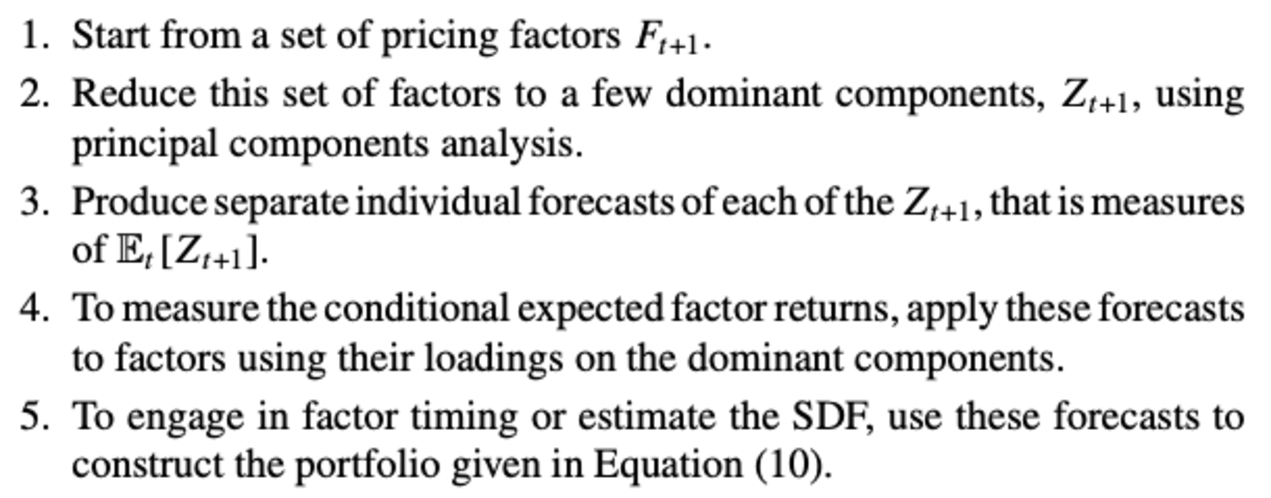
\includegraphics[width=300pt]{Steps.pdf}
	\end{figure}
\end{frame}

\begin{frame}{Methodology}
	\begin{itemize}
		\item Use fifty `anomaly' portfolios from Kozak et al. (2020)\footnote{\tiny Kozak, S., S. Nagel, and S. Santosh. 2020. Shrinking the cross-section. \textit{Journal of Financial Economics} 135:271–92.} that effectively capture market heterogeneity.
		\begin{itemize}
			\item These anomalies are the usual anomalies like Size, Value, ROA, SUE, etc.
		\end{itemize}
		\item Break them into deciles, create long-short portfolios for each anomaly (Decile 10 minus Decile 1).
		\begin{itemize}
			\item For each portfolio, they calculate the market-cap-weighted book-to-market ratio ($bm$) of the underlying stocks.
			\item By finding the difference in log book-to-market of Portfolio 10 minus that of Portfolio 1.
		\end{itemize}
	\end{itemize}
\end{frame}

\begin{frame}{Methodology}
	\begin{itemize}
		\item Market-adjust and rescale the data. 
		\begin{enumerate}
			\item Calculate regression $\beta$ for each anomaly. 
			\item Market-adjust returns and predictors by subtracting $\beta \times r_{mkt}$ for returns and $\beta \times bm_{mkt}$ for $bm$ ratios.
			\item Rescale to equalize the variance of market-adjiusted returns, and $bm$ ratios for each anomaly.
		\end{enumerate}
		\item So now they have 50 long-short portfolios and their corresponding $bm$ ratios.
	\end{itemize}
\end{frame}

\begin{frame}{Methodology}
	\begin{itemize}
		\item They conduct a PCA to reduce the 50 long-short portfolios to five PCs that explain roughly 60\% of the variance.
		\begin{figure}[!ht]
		\centering
			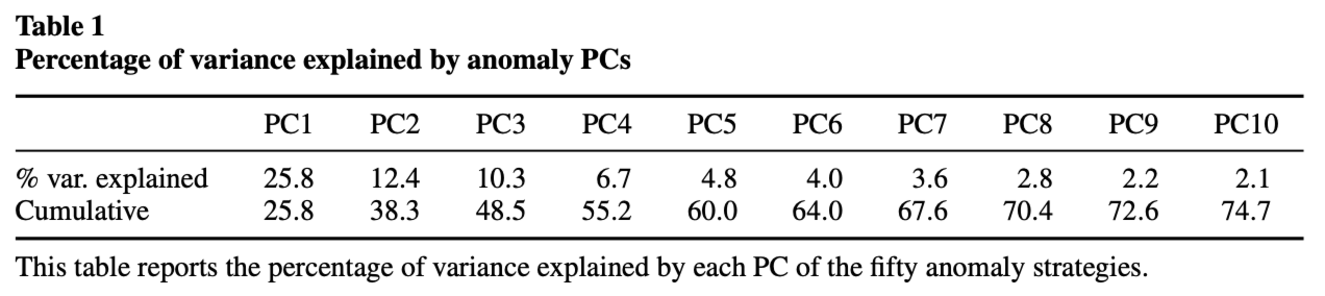
\includegraphics[width=250pt]{Table1.pdf}
		\end{figure}
		\item Why five? 
		\begin{enumerate}
			\item Campbell and Thompson (2007)\footnote{\tiny Campbell, J. Y., and S. B. Thompson. 2007. Predicting excess stock returns out of sample: Can anything beat the historical average? \textit{Review of Financial Studies} 21:1509–31.} show that the monthly $R^2$ when predicting the market is around 75bp.
			\item A loose upper-bound on the annual Sharpe is 1, or 8.3\% monthly. 
		\end{enumerate}
		\item If each included PC contributes equally to the $R^2$, the harmonic mean of their contribution to the total variance of returns must be $> \frac{0.75}{8.3} \approx 9\%$.
	\end{itemize}
\end{frame} 

\begin{frame}{Methodology}
	\begin{itemize}
		\item Construct the $bm$ portfolios for the each PC by combining anomaly-portfolio log $bm$s according to portfolio weights:
		\begin{equation}
			bm_{i,t} = q^\prime_t bm_t^F
		\end{equation}
		\item where 
		\begin{itemize}
			\item $q_i$ is the $i$-th column of $Q$, the matrix of eigenvectors, and $F$ is the anomaly.
			\item Use the difference between this quantity for the long and short leg of the PCs.
		\end{itemize}
		\item Analyze the predictability using monthly holding periods.
	\end{itemize}
\end{frame}

\begin{frame}{Results}
	\begin{figure}[!ht]
	\centering
		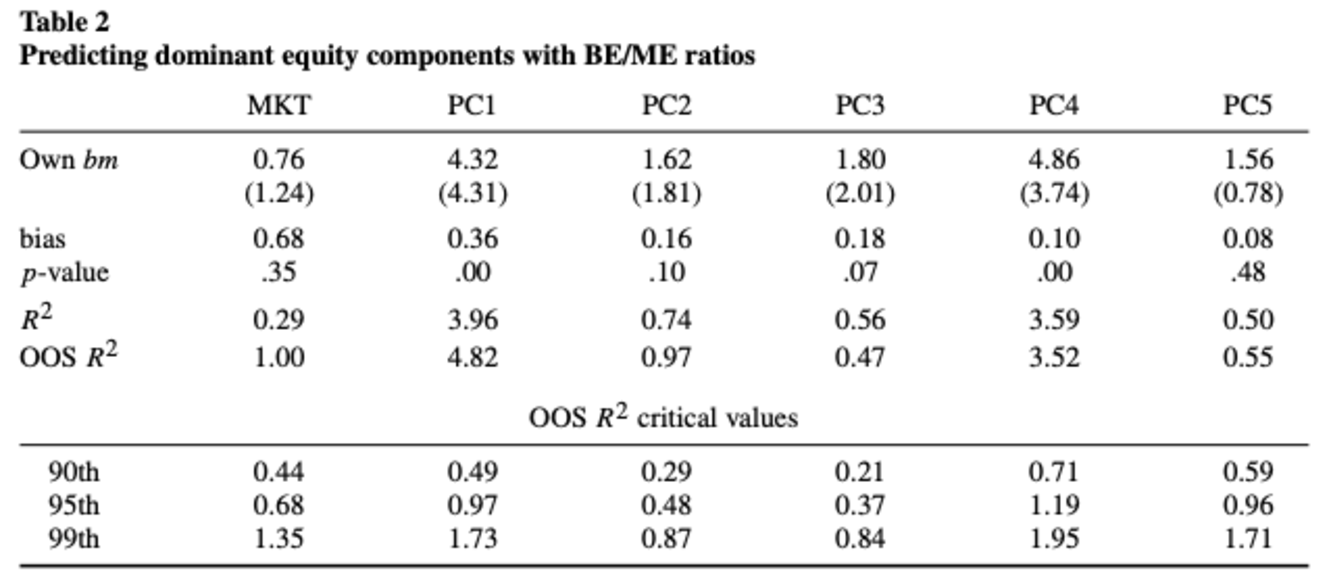
\includegraphics[width=300pt]{Table2.pdf}
	\end{figure}
\end{frame}

\end{document}